\chapter{Introduction}

Modelling cetacean (whale, dolphin, and porpoise) population dynamics and behaviour is paramount to effective population management and conservation. Robust data is required for the design and implementation of conservation strategies and to assess the risks presented by anthropogenic activity such as offshore wind turbines and commercial fishing. Moreover, cetaceans make prime candidates for modelling ecosystem change under the ecosystem sentinel concept as they reflect the current state of the ecosystem and respond to change across different spatial and temporal scales \cite{moore_marine_2008}. As the global climate changes and urbanisation of coastal areas intensifies, it is imperative to develop methodologies for quick and effective assessment of the biological and ecological impact of rising sea temperatures, pollution, and habitat degradation. This can be achieved through modelling the population, behaviour, and health of large marine species such as dolphins.

Methodologies of cetacean research includes photo identification (photo-id). Photo-id involves collecting photographic data and identifying individuals based on unique permanent markings, and has been used for more than 40 years for modelling cetacean population dynamics and ecology \cite{connor_male_2015, wursig_photographic_1977}. Current identification techniques for cetaceans rely heavily on experts manually identifying individuals. This can often be costly due to the number of person-hours required for identification, as well as the large potential for error due to issues such as observer fatigue. Further, individual identification of dolphins within a species is time consuming due to the nature of the task. Intra-species dolphins have very similar markings and body types making identifying an individual within a pod very difficult. Prominent features must be identified, such as small nicks to the fins or scars left from injuries to identify an individual. If these features are only prominent on one side of the individual, the task of identification becomes even more difficult.

\begin{figure}[H]
	\begin{center}
		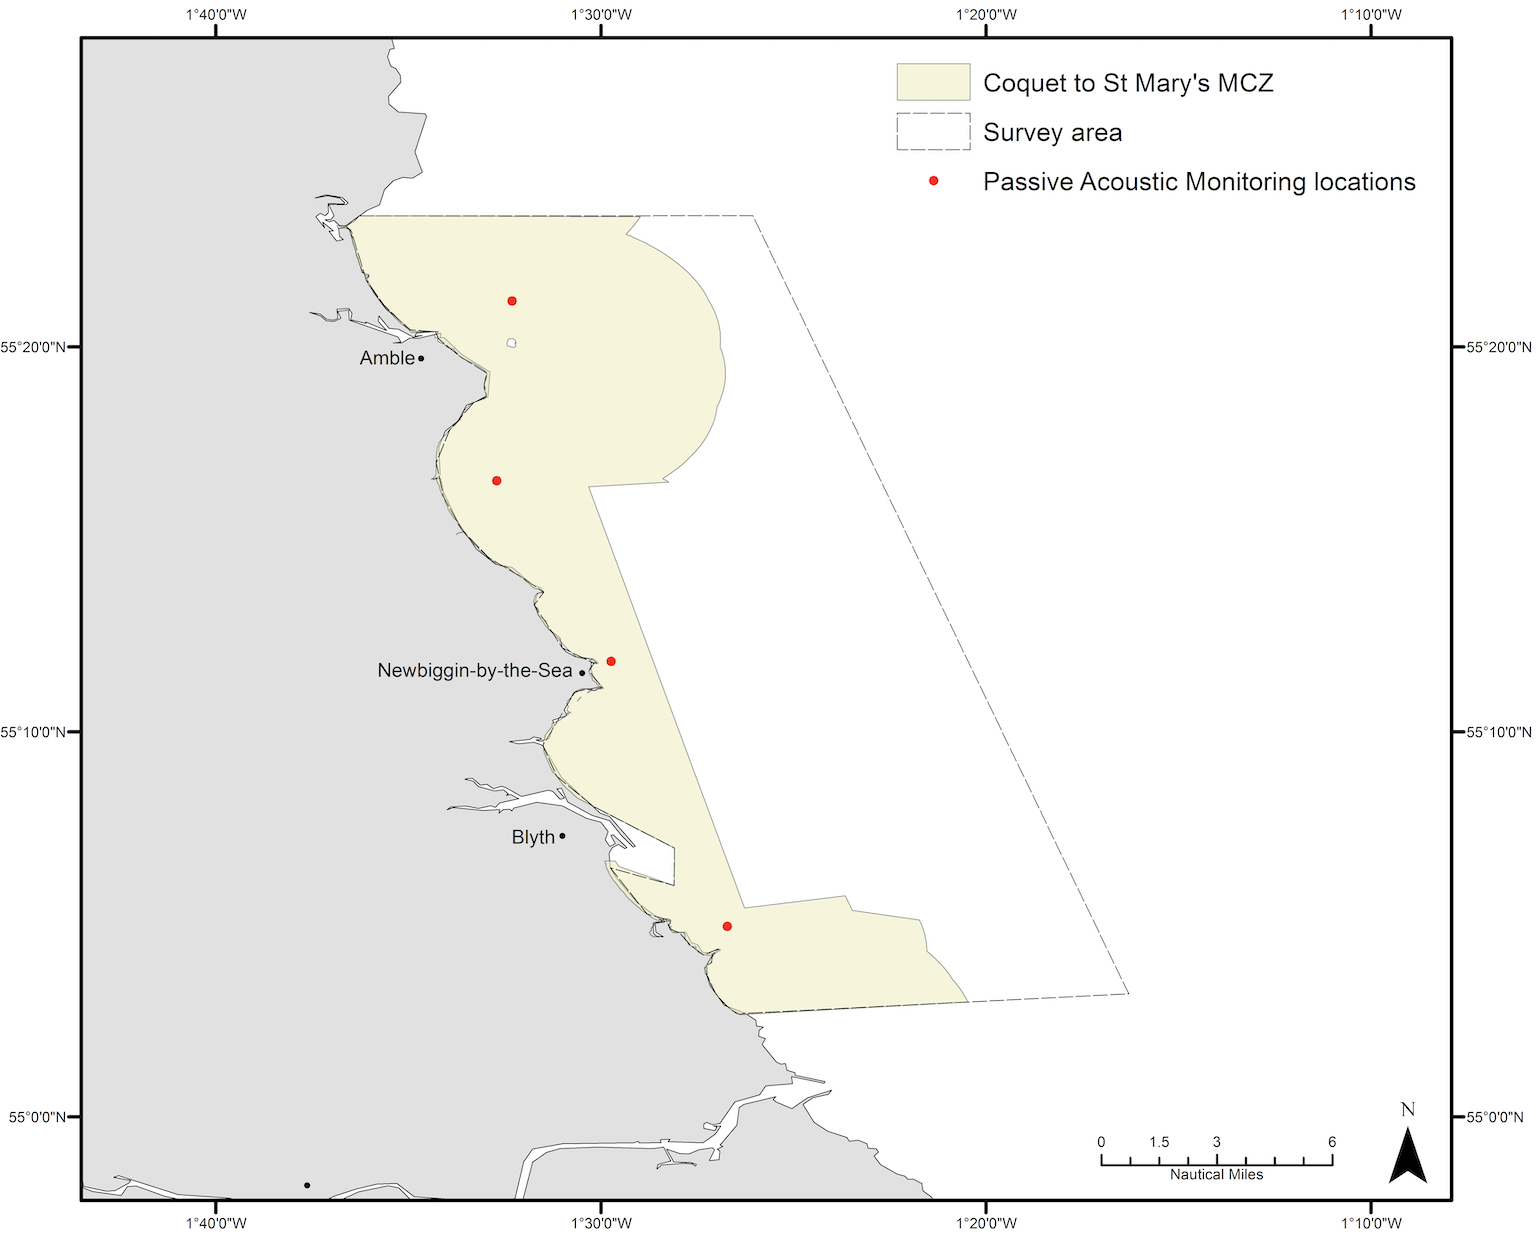
\includegraphics[width=\linewidth]{Chapter1/figs/map.png}
	\end{center}
	\caption{Map of the survey area, Northumberland, UK, from St. Mary's Lighthouse in the south to 25nm above Coquet Island in the north.}
	\label{fig:map}
\end{figure}

With progressively more data being collected during fieldwork through increased use of technology, there is an urgent need for an automatic system for quick identification with reduced error rates. Previous efforts to photo-id individuals from underwater video stills from previous expeditions undertaken by Newcastle University's School of Natural \& Environmental Science's Marine MEGAfauna Lab took around three months from raw video file to be completely catalogued. This project addresses these limitations by applying the methodologies, techniques, and computational power of deep learning to the field of marine biology. Deep learning models, specifically Convolutional Neural Networks (CNNs), will be trained on high-end computer clusters using the Microsoft Azure Cloud\footnote{Microsoft Azure Cloud: \href{http://azure.microsoft.com}{azure.microsoft.com}} prior to field studies using existing data. Once trained, the models can be ran on field deployable computers to perform image analysis in real time from multiple data sources (underwater and above water images, and aerial drone footage). Methodologies incorporating these models are be designed to quickly identify individuals, assess health, analyse behaviour and incorporate remote sensing techniques. 

CNNs have for many years now been regarded as the main approach for solving image and computer vision related problems. More recently, the development of deep-layered CNNs and the availability of  high-powered GPUs have provided the perfect platform for solving fine-grained computer vision tasks. This project has developed a system to speed up marine cetacean photo-id using a pipeline of CNNs. Starting with a large high resolution image, this pipeline allows for the detection and identification of cetaceans in the image. This system can greatly aid marine biologists, speeding up the identification process allowing for more time to be spent on developing response strategies and health assessments. 

Data collection for this project focussed on a population of white-beaked dolphins (\textit{Lagenorhynchus albirostris}) off the coast of North-East England (see Figure \ref{fig:map}). Recent research has identified sites where the species is regularly sighted \cite{galatius_lagenorhynchus_2016, hammond_cetacean_nodate} and underwater image analysis has shown seasonal and multi-year residency. A health assessment based on underwater image analysis identified high incidence of skin disease and trauma suggesting conservation of this population should be high priority \cite{van_bressem_visual_2018}. The species would also serve as a prime sentinel for monitoring North Sea climatic changes as it shows preference for cold water with North-East UK coastal waters representing the southern limit of its range.

\section{Research Problem}

\section{Contributions}

\section{Thesis Structure}

\section{Related Publications}


%%%%%%%%%%%%%%%%%%%%%%%%%%%%%%%%%%
